\documentclass{ximera}

\usepackage{gensymb}
\usepackage{tabularx}
\usepackage{mdframed}
\usepackage{pdfpages}
%\usepackage{chngcntr}

\let\problem\relax
\let\endproblem\relax

\newcommand{\property}[2]{#1#2}




\newtheoremstyle{SlantTheorem}{\topsep}{\fill}%%% space between body and thm
 {\slshape}                      %%% Thm body font
 {}                              %%% Indent amount (empty = no indent)
 {\bfseries\sffamily}            %%% Thm head font
 {}                              %%% Punctuation after thm head
 {3ex}                           %%% Space after thm head
 {\thmname{#1}\thmnumber{ #2}\thmnote{ \bfseries(#3)}} %%% Thm head spec
\theoremstyle{SlantTheorem}
\newtheorem{problem}{Problem}[]

%\counterwithin*{problem}{section}



%%%%%%%%%%%%%%%%%%%%%%%%%%%%Jenny's code%%%%%%%%%%%%%%%%%%%%

%%% Solution environment
%\newenvironment{solution}{
%\ifhandout\setbox0\vbox\bgroup\else
%\begin{trivlist}\item[\hskip \labelsep\small\itshape\bfseries Solution\hspace{2ex}]
%\par\noindent\upshape\small
%\fi}
%{\ifhandout\egroup\else
%\end{trivlist}
%\fi}
%
%
%%% instructorIntro environment
%\ifhandout
%\newenvironment{instructorIntro}[1][false]%
%{%
%\def\givenatend{\boolean{#1}}\ifthenelse{\boolean{#1}}{\begin{trivlist}\item}{\setbox0\vbox\bgroup}{}
%}
%{%
%\ifthenelse{\givenatend}{\end{trivlist}}{\egroup}{}
%}
%\else
%\newenvironment{instructorIntro}[1][false]%
%{%
%  \ifthenelse{\boolean{#1}}{\begin{trivlist}\item[\hskip \labelsep\bfseries Instructor Notes:\hspace{2ex}]}
%{\begin{trivlist}\item[\hskip \labelsep\bfseries Instructor Notes:\hspace{2ex}]}
%{}
%}
%% %% line at the bottom} 
%{\end{trivlist}\par\addvspace{.5ex}\nobreak\noindent\hung} 
%\fi
%
%


\let\instructorNotes\relax
\let\endinstructorNotes\relax
%%% instructorNotes environment
\ifhandout
\newenvironment{instructorNotes}[1][false]%
{%
\def\givenatend{\boolean{#1}}\ifthenelse{\boolean{#1}}{\begin{trivlist}\item}{\setbox0\vbox\bgroup}{}
}
{%
\ifthenelse{\givenatend}{\end{trivlist}}{\egroup}{}
}
\else
\newenvironment{instructorNotes}[1][false]%
{%
  \ifthenelse{\boolean{#1}}{\begin{trivlist}\item[\hskip \labelsep\bfseries {\Large Instructor Notes: \\} \hspace{\textwidth} ]}
{\begin{trivlist}\item[\hskip \labelsep\bfseries {\Large Instructor Notes: \\} \hspace{\textwidth} ]}
{}
}
{\end{trivlist}}
\fi


%% Suggested Timing
\newcommand{\timing}[1]{{\bf Suggested Timing: \hspace{2ex}} #1}




\hypersetup{
    colorlinks=true,       % false: boxed links; true: colored links
    linkcolor=blue,          % color of internal links (change box color with linkbordercolor)
    citecolor=green,        % color of links to bibliography
    filecolor=magenta,      % color of file links
    urlcolor=cyan           % color of external links
}

\title{Arithmetic Series}
\author{Bart Snapp and Brad Findell}

\outcome{Sum arithmetic series.}

\begin{document}
\begin{abstract}
We study arithmetic series.
\end{abstract}
\maketitle

\label{A:arithmeticSeries}

In this activity, we explore \emph{arithmetic series}, which are sums of consecutive terms from an arithmetic sequence.

Ms. Nguyen's math class has been looking at ``triangular numbers.''  The first 6 triangular numbers are shown below. 
\begin{image}
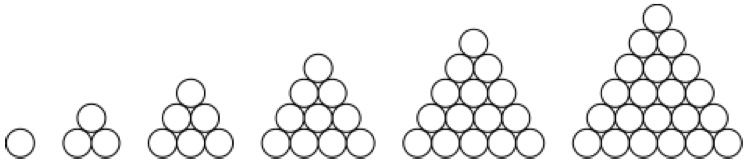
\includegraphics{triangularNumbers} % Need an original graphic.
\end{image}

\begin{teachingnote}
Consider starting this problem without help.  Then students can 
compare the following collection of solutions with the solution(s) that they came up with on their own. 
\end{teachingnote}

\begin{problem}
Blair wanted to find the $551^{st}$ triangular number.  She used a table and looked for a pattern in the \emph{sequence of partial sums}:  $1, 1+2, 1+2+3, \dots$.  Help her finish her idea.  
\end{problem}

\begin{problem}
Kaley realized the the $551^{st}$ triangular number would be the sum 
\[
1+2+3+4+\dots+548+549+550+551
\]
She started pairing the first with the last number; the second with the second-to-last; the third with the third-to-last; and so on.  She saw that the averages are always the same.  Help her finish her idea.  
\end{problem}

\begin{problem}
Ali begin by writing out the sum forward and backward and follows:  
\[
\begin{array}{c@{ + }c@{ + }c@{ + }c@{ + }c@{ + }c@{ + }c@{ + }c@{ + }c@{ + }c@{ + }c@{ + }c@{ + }c}
1 & 2 & 3 & 4 & 5 & 6 & \cdots & 546 & 547 & 548 & 549 & 550 & 551 \\
551 & 550 & 549 & 548 & 547 & 546 & \cdots & 6 & 5 & 4 & 3 & 2 & 1 
\end{array}
\]
Help her finish her idea.  Be sure to explain clearly what happens ``in the dots.''  Does it matter whether there are an even or an odd number of terms?  
\end{problem}

\begin{problem}
Cooper was interested in a different triangular number and drew the following picture:   
\begin{image}
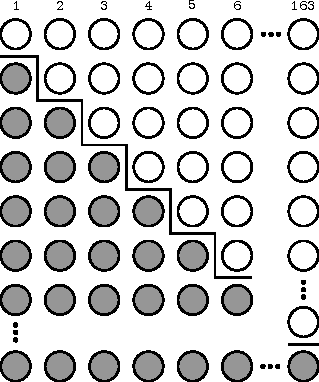
\includegraphics{sum1.pdf}
\end{image}
Which triangular number was he finding?  Help him finish his idea.  Be sure to explain clearly what 
happens ``in the dots.'' 
\end{problem}


\begin{problem}
Sum the numbers:  
\[
106 + 112 + 118 + \dots + 514
\]
\end{problem}

\begin{problem}
Sum the numbers:
\[
2.2 + 2.9 + 3.6 + 4.3 + \dots + 81.3
\]
\end{problem}


\begin{problem}
Suppose you have an arithmetic sequence beginning with $a$, with a constant difference of $d$ and with $n$ terms.  
\begin{enumerate}
\item What is the $n^{th}$ term of the sequence?  
\item Use dots to write the series consisting of the first $n$ terms of this sequence.
\item Find the sum of this series.  
\end{enumerate}
\end{problem}

\end{document}
